\documentclass[a4paper,twoside,12pt]{scrbook}
\usepackage{amsmath}
\usepackage{amssymb,amsthm,mathtools}
\usepackage[utf8]{inputenc} 
\usepackage[hang,font={small,sl},hang,labelfont=bf]{caption}
\usepackage[font+={footnotesize}]{subcaption}
\usepackage[dvipsnames]{xcolor}
\usepackage{calc}
\usepackage{longtable} % tables over several pages
\usepackage{supertabular}
\usepackage{array}
\usepackage{algpseudocode}
\usepackage{algorithm}
\usepackage{booktabs} % publication quality tables for LaTeX
\usepackage{multicol}
\usepackage{breqn}
\usepackage{soul}
\ifpdfoutput{%
	\usepackage[pdftex]{graphicx}
	\usepackage[]{pdfpages} %for including full pdf pages
}{%
	\usepackage{graphicx}
}
\usepackage{epstopdf}
\usepackage{tikz}
\usetikzlibrary{matrix, positioning,patterns, shapes.misc}
\usepackage{pgfplots}
\usepgfplotslibrary{groupplots}
\usepackage{pgfplotstable}
\epstopdfsetup{update} % only regenerate pdf files when eps file is newer
\usepackage{rotating} % rotate figures
\usepackage[headinclude]{scrpage2}
% Font packages:
\usepackage{times}
\usepackage{helvet}
\usepackage[T1]{fontenc}

\ifpdfoutput{%
	\usepackage[pdftex,
		bookmarks,
		bookmarksopen=true,
		bookmarksnumbered=true,
		pdfauthor={Sephora Madjiheurem},
		pdftitle={Deep spatio-temporal structural model for action recognition},% RENAME?
		colorlinks,
		linkcolor=darkgray,
		citecolor=MidnightBlue,
		filecolor=black,
		urlcolor=NavyBlue,
		anchorcolor=black,
		menucolor=black,
		breaklinks=false,
		pageanchor=true,
		plainpages=false,
		pdfpagelabels=true]{hyperref}
	\usepackage{url}
}{}

\ifpdfoutput{%
	\pdfcompresslevel=9
	\pdfoutput=1
	\DeclareGraphicsExtensions{.pdf,.png}
}{}

\bibliographystyle{amsplain}

\RedeclareSectionCommand[beforeskip=20ex, afterskip=2cm]{chapter}

% A4
%
\topmargin -0.5in
\textheight 9.3in
\textwidth 6.3in
\oddsidemargin 0.18in
\evensidemargin -0.22in
\parskip 0.1in
\parindent 0in

\renewcommand{\arraystretch}{1.5}
\renewcommand{\baselinestretch}{1}

% !TEX root = ../thesis.tex
\graphicspath{{figures/}}
\newcommand*{\TODO}{\mbox{\large\bf TO DO}}
\newcommand*{\REFR}{\mbox{\large\bf REFR}}
\newcommand*{\x}{\mathbf{x}}
\newcommand*{\w}{\mathbf{w}}
\renewcommand*{\v}{\mathbf{v}}
\DeclareMathOperator*{\argmin}{arg\,min}
\DeclareMathOperator*{\argmax}{arg\,max}
\DeclareMathOperator*{\wrt}{d\,}
\newcommand*\derivative[2]{\dfrac{\partial #1}{\partial #2}}
\newcommand*\rfrac[2]{{}^{#1}\!/_{#2}}%running fraction with slash - requires math mode.
%  Terminates current page and paragraph, makes sure next page starts on
%  an odd-number, and generates a completely blank page, without page markers,
%  if necessary.
\newcommand{\clearemptydoublepage}{\newpage{\pagestyle{empty}\cleardoublepage}}

% svg
\makeatletter
\g@addto@macro\@verbatim\small
\makeatother 

\newcommand{\executeiffilenewer}[3]{%
 \ifnum\pdfstrcmp{\pdffilemoddate{#1}}%
 {\pdffilemoddate{#2}}>0%
 {\immediate\write18{#3}}\fi%
}

\newcommand{\includesvg}[1]{%
 \executeiffilenewer{#1.svg}{#1.pdf}%
 {inkscape -z -D --file=#1.svg %
 --export-pdf=#1.pdf --export-latex}%
 \input{#1.pdf_tex}%
}
\newcommand{\algorithmautorefname}{Algorithm}
\algnewcommand\Continue{\State\textbf{continue}}
\algnewcommand\Break{\State\textbf{break}}
\makeatletter
\algnewcommand{\NewLine}{\Statex \hskip\ALG@thistlm}
\algnewcommand{\LineComment}[1]{\Statex \hskip\ALG@thistlm \(\triangleright\) #1}
\makeatother

\newcolumntype{M}[1]{>{\centering\arraybackslash}m{#1}}
\newcolumntype{P}[1]{>{\centering\arraybackslash}p{#1}}
% plots
\pgfplotsset{
compat=1.5,
every tick label/.append style={font=\footnotesize}, 
every legend/.append style={font=\footnotesize},
enlargelimits=false,
every label/.append style={
/pgf/number format/fixed,
/pgf/number format/precision=2
},
scaled y ticks=false,
/pgfplots/ybar legend/.style={
/pgfplots/legend image code/.code={%
\draw[##1, bar width=3pt,yshift=-0.2em,bar shift=0pt]
plot coordinates {(0cm,0.5em)};},
},
every axis title/.append style={font=\small},
every axis label/.append style={font=\footnotesize},
unbounded coords=jump,
group style={x descriptions at=edge bottom,
y descriptions at=edge left},
}

\pgfplotstableset{% global config, for example in the preamble
% these columns/<colname>/.style={<options>} things define a style
% which applies to <colname> only.
empty cells with={--}, % replace empty cells with ’--’
every head row/.style={before row=\hline,after row=\hline},
every last row/.style={after row=\hline},
precision=2,fixed zerofill,fixed,
%column type/.add={|}{},% results in ’|c’,
every first column/.style={string type, column type/.add={|}{|}},
every last column/.style={
column type/.add={}{|}
},
}
% multicol supertabular
\newcount\n
\n=0
\def\tablebody{}
\makeatletter
\loop\ifnum\n<300
        \advance\n by1
        \protected@edef\tablebody{\tablebody
                \textbf{\number\n.}&
                \hfill T\hfill\hfill F\hfill\hskip0pt\endgraf
                \vskip.5\baselineskip
                \color@begingroup
                \color{black!20}
                \hrule height3ex
                \color@endgroup
                \tabularnewline
        }
\repeat
\makeatother
% !TEX root = ../thesis.tex

% Stripped from acm siggraph bst and cls
\makeatletter

% no labels in bibliography.
%\def\@biblabel#1{}

%\newlength{\bibhang}
%\setlength{\bibhang}{1em}

% Change in-bibliography biberence style
%\def\thebibliography#1{%
%  \section*{%
 %   \bibname\@mkboth{\sl\uppercase{\bibname}}{\sl\uppercase{\bibname}}}
  %\list{\relax}{\setlength{\labelsep}{0em}
   %             \setlength{\itemindent}{-\bibhang}
    %            \setlength{\leftmargin}{\bibhang}}
 % \def\newblock{\hskip .11em plus .33em minus .07em}
 % \sloppy\clubpenalty4000\widowpenalty4000
 % \sfcode`\.=1000\relax}

% Change in-document citation styles
\let\@internalcite\cite
\def\cite{\def\citename##1{##1}\@internalcite}
\def\shortcite{\def\citename##1{}\@internalcite}

\makeatother


\begin{document}

%% Define leading chapter pages

% !TEX root = ../thesis.tex
\addtokomafont{paragraph}{\sffamily}

\def\mychpstyleintl{%
{\noindent\setlength{\tabcolsep}{0pt}\setlength{\arrayrulewidth}{2pt}%
\begin{tabular}{c}
\\[10ex]
\begin{tabular}{lr}
\begin{tabular}{p{0.6\linewidth}}
\\
\end{tabular}
&
\begin{tabular}{p{0.4\linewidth}}
	\begin{flushright}
\rightline{{%
		\sffamily%
		\fontseries{bx}%
		\fontshape{n}%
		\fontsize{100}{120}%choose baselineskip to be 1.2 times font size
		\selectfont
		\thechapter}}		
	\end{flushright}

\end{tabular}
\end{tabular}\\[300pt]
\end{tabular}
}}
\newpagestyle{mychapterpagestyle}{{\protect\mychpstyleintl}{\protect\mychpstyleintl}}{}
\newpagestyle{myappendixpagestyle}{{\protect\mychpstyleintl}{\protect\mychpstyleintl}}{}
%%

%refs
%\newcommand{\chpref}[1]{Chapter \ref{#1}}
%\newcommand{\secref}[1]{Section \ref{#1}}
%\newcommand{\figref}[1]{Figure \ref{#1}}
%\newcommand{\tabref}[1]{Table \ref{#1}}
%\newcommand{\apxref}[1]{Appendix \ref{#1}}
%%

% --- selfmade version ----
\begin{titlepage}
	\topmargin 1.0cm
	\oddsidemargin 0.0cm
	\evensidemargin 0.0cm
	%\textwidth 6.5in
	\centering
	\Huge
	\vspace{3.0cm}
	\textbf{\textsf{Deep spatio-temporal structural model for free-form action recognition}} \\[2.0cm]
%\begin{figure}[h]\centering
%\begin{subfigure}{0.16\linewidth}
%\includegraphics[width=\columnwidth]{figures/babycrawling.png}
%\end{subfigure}%
%\begin{subfigure}{0.16\linewidth}
%\includegraphics[width=\columnwidth]{figures/handstandwalking.png}
%\end{subfigure}%
%\begin{subfigure}{0.16\linewidth}
%\includegraphics[width=\columnwidth]{figures/pushup.png}
%\end{subfigure}%
%\begin{subfigure}{0.16\linewidth}
%\includegraphics[width=\columnwidth]{figures/pizzatossing.png}
%\end{subfigure}%
%\begin{subfigure}{0.16\linewidth}	    \includegraphics[width=\columnwidth]{figures/playingviolin.png}
%\end{subfigure}%
%\begin{subfigure}{0.16\linewidth}
%\includegraphics[width=\columnwidth]{figures/archery.png}
%\end{subfigure}
%\begin{subfigure}{0.16\linewidth}
%\includegraphics[width=\columnwidth]{figures/frontcrawl.png}
%\end{subfigure}%
%\begin{subfigure}{0.16\linewidth}
%\includegraphics[width=\columnwidth]{figures/surfing.png}
%\end{subfigure}%
%\begin{subfigure}{0.16\linewidth}
%\includegraphics[width=\columnwidth]{figures/skydiving.png}
%\end{subfigure}%
%\begin{subfigure}{0.16\linewidth}
%\includegraphics[width=\columnwidth]{figures/bowling.png}
%\end{subfigure}%
%\begin{subfigure}{0.16\linewidth}
%\includegraphics[width=\columnwidth]{figures/balancebeam.png}
%\end{subfigure}%
%\begin{subfigure}{0.16\linewidth}
%\includegraphics[width=\columnwidth]{figures/writingonboard.png}
%\end{subfigure}
%\end{figure}
	\vspace{3cm}
	\sffamily
	\Large
	Sephora Madjiheurem
	\\[0.8cm]
	\large
	Master Thesis
	\\
	April 2016
	\\[1.3cm]
	\emph{Supervisors:}\\
	Jie Song\\
	Dr.\ Mathieu Salzmann\\
	Prof.\ Dr.\ Otmar Hilliges		% The supervising professor
	\vfill
	\includegraphics*[height=0.8cm]{figures/eth_logo_kurz_pos.eps} \hfill
	\includegraphics*[height=0.8cm]{figures/logo-ait}
	\vspace{3.4cm}
\end{titlepage}
\clearemptydoublepage
%%

\pagenumbering{roman}
\setcounter{page}{1}

\chapter*{Abstract}
Human action is a high-level concept in computer vision research and understanding it may benefit from different semantics, such as human pose, interacting objects, and scene context.

In this thesis, we explicitly exploit semantic cues with aid of existing object detectors for action recognition in videos, and thoroughly study their effect on the recognition performance for different types of actions. 

Specifically, we propose a new deep architecture by incorporating object/human detection results into the framework for action recognition.

Our proposed architecture not only shares great modeling capacity with two-stream input augmentation, but also exhibits the flexibility of leveraging semantic cues (e.g. scene, person, object) for action understanding.

We perform experiments on UCF101 dataset and demonstrate its superior performance to the original two-stream CNN.
In addition, we systematically study the effect of incorporating semantic cues on the recognition performance for different types of action classes, and try to provide some insights for building more reasonable action benchmarks and robust recognition algorithms.

%-----------------------------------------------------------------------------------------------
%include task description here:
%\cleardoublepage
%-----------------------------------------------------------------------------------------------

%include acknowledgment here:
% !TEX root = ../thesis.tex

\chapter*{Ackowledgement}
I would like to express my sincere gratitude to my supervisor Jie Song. His continuous guidance and boundless patience has given me immense inspiration and courage. 

My sincere thanks also goes Dr.Limin Wang, whose insightful advice was crucial for the major breakthroughs in this thesis.

The completion of this thesis also owes to the tremendous love and care from my precious friends.

Especially, I would like to thank Srivathsan Murali, Seon-Wook Park for their endless encouragement and unconditioned help. 
Working beside you has been a great honour and your dedication to work has been a constant motivation for me.\newline 
To Pavol Vyhlidal, who taught me never cease to confront personal boundaries and take on new challenges in life.\newline
To Federico Danieli, who has accompanied me through my ups and downs.
Your valuable opinions gave rise to numerous progress; your loving support has been the greatest fuel that drove me forward.

Last but not least, I am thankful to my family. You enabled everything, EVERYTHING.
\setcounter{tocdepth}{1}
\tableofcontents

\cleardoublepage
\phantomsection
\addcontentsline{toc}{chapter}{List of Figures}
\listoffigures

\cleardoublepage
\phantomsection
\addcontentsline{toc}{chapter}{List of Tables}
\listoftables
\cleardoublepage

\pagenumbering{arabic}
\renewcommand*{\chapterpagestyle}{mychapterpagestyle}
\renewcommand*{\chapterformat}{} % show chapter titles only (no numbers)
\renewcommand*{\sectionformat}{\thesection\enskip\enskip}
\renewcommand*{\subsectionformat}{\thesubsection\enskip}
\renewcommand*{\tableformat}{\tablename~\thetable}
\renewcommand*{\figureformat}{\figurename~\thefigure}
\captionsetup{subrefformat=parens}

% ---- TABLES ----
\pgfplotstableread[col sep=comma,
assume math mode,
columns/category/.style={reset styles, string type},
]{data/map_cate.dat}{\mapcatedat}
\pgfplotstableread[
columns/name/.style={reset styles, string type},
columns/flowname/.style={reset styles, string type}
]{data/top_10_growth.dat}{\toptengrowth}
\pgfplotstableread[
columns/name/.style={reset styles, string type},
columns/flowname/.style={reset styles, string type}
]{data/top_10_reduce.dat}{\toptenreduce}
\pgfplotstableread[
columns/name/.style={reset styles, string type},
]{data/temporal5perc.dat}{\temporalgains}
\pgfplotstableread[
columns/name/.style={reset styles, string type},
]{data/spatial5perc.dat}{\spatialgains}
\pgfplotstableread[col sep=comma,
assume math mode,
columns/category/.style={reset styles, string type}
]{data/pos_channel.dat}{\poschanneldat}
\pgfplotstableread[
assume math mode,
columns/name/.style={reset styles, string type},
]{data/hointeraction.dat}{\interactiondat}
\pgfplotstableread[col sep=comma,
assume math mode,
columns/category/.style={reset styles, string type}
]{data/ps_channel.dat}{\pschanneldat}
% ---- MAIN PART ----

% !TEX root = ../thesis.tex

% set counter to n-1:
\setcounter{chapter}{0}

\chapter{Introduction}\label{chap:intro}
\section{Action Recognition}
Video based action recognition finds its usage in a broad range of practical applications such as surveillance, video analysis and retrieval as well as human computer interaction. In the recent years, evidently increasing research effort has been devoted in this topic. However, despite the intense research, it remains one of the unconquered fields in computer vision.

The two major milestones are marked with the development of a series of trajectory based feature extractor \cite{wang2011action,wang2013action} and the success application of deep neural network in action recognition \cite{simonyan2014two}. 
The former, typically used in the standard Bag of Visual Words (BoVW) pipeline together with advanced encoding method \cite{perronnin2010improving, peng2014action}, is broadly used as benchmark for later methods. 
Meanwhile the latter, the first Convolutional Neural Network (CNN) \cite{lecun1989backpropagation} based approach that yielded competitive performance, stimulated many valuable follow-up proposals with various focuses oriented on improvements for deployment of deep neural network in action recognition \cite{wang2015temporal,xiong2015recognize}.

However, as video datasets become more and more challenging, the performance of CNN based methods seem to have reached a bottleneck. 
In particular, as video clips gets more realistic and the temporal trimming more fuzzy, the definition of "action" demands a second thought. 

On one hand, an action is a series of events connected in time, recognizing an action often requires consideration of temporal evolution. 
The original CNN tackles this issue by applying a simple temporal pooling on the frame-wise classification results, which becomes an apparent weakness when dealing with long untrimmed video sequences. 
In order to tackle this drawback, 3D-CNN \cite{ji20133d} as well as LSTM (Long Short Term Memory) Models \cite{donahue2015long,yue2015beyond} have been opted to emphasize the evolvement in time. 
However, given the complexity of their architectures, the performance yielded by such approaches are harshly jeopardized by the inadequacy of available datasets.

On the other hand, the recognition of an action in video can be seen as an interplay of recognizing different components of an event. 
In fact, for many action categories one does not even need any temporal evolution to classify them; as is shown in \autoref{fig:singleframe}, one can easily classify the whole video sequence given the composition of objects or scene in a single frame. 
As a matter of fact, this concept has already been widely implemented and intensely optimised in low-level features, primarily by applying various fusion techniques \cite{peng2014bag} on descriptors from different cues such as Histogram of Gradients (HOG) \cite{laptev2008learning} for appearance cue and Motion Boundary Histogram (MBH) \cite{wang2013action} for motion cue. However on semantic level this field still remains scarce. 

\begin{figure}
\centering
\begin{subfigure}{0.30\textwidth}
	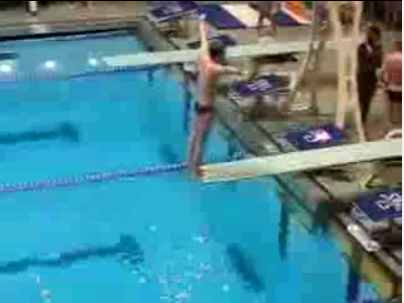
\includegraphics[height=3cm, width=4cm, keepaspectratio=false]{figures/scene_domi0.png}
\caption{Scene}\label{fig:scenedomi}
\end{subfigure}
\begin{subfigure}{0.30\textwidth}
	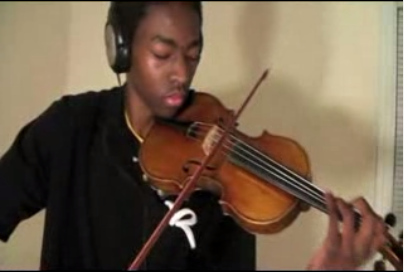
\includegraphics[height=3cm, width=4cm,]{figures/obj_domi0.png}
\caption{Object}\label{fig:objdomi}
\end{subfigure}
\caption[Scene and object centric videos]{Sample frames from UCF101 dataset, where perceptually the appearance of scene or objects is sufficient for correct recognition of an action class.}\label{fig:singleframe}
\end{figure}

\begin{figure}
\begin{subfigure}{0.5\linewidth}
\begin{tikzpicture}[nodes={font=\footnotesize,anchor=center}]
\node[inner sep=0pt] (h1) at (0,0)
    {\includegraphics[width=.3\columnwidth]{figures/babycrawling.png}};
\node[below] at (h1.south){BabyCrawling};
\node[right=0pt of h1,inner sep=0pt] (h2)
    {\includegraphics[width=.3\columnwidth]{figures/handstandwalking.png}};
\node[below] at (h2.south){Handstand};
\node[right=0pt of h2, inner sep=0pt] (h3)
    {\includegraphics[width=.3\columnwidth]{figures/pushup.png}};
\node[below] at (h3.south){PushUp};
\end{tikzpicture}
\caption{Body Motion Only}
\end{subfigure}
\begin{subfigure}{0.5\linewidth}
\begin{tikzpicture}[nodes={font=\footnotesize,anchor=center}]
\node[inner sep=0pt] (h1) at (0,0)
    {\includegraphics[width=.3\columnwidth]{figures/pizzatossing.png}};
\node[below] at (h1.south){PizzaTossing};
\node[right=0pt of h1,inner sep=0pt] (h2)
    {\includegraphics[width=.3\columnwidth]{figures/playingviolin.png}};
\node[below] at (h2.south){PlayingViolin};
\node[right=0pt of h2, inner sep=0pt] (h3)
    {\includegraphics[width=.3\columnwidth]{figures/archery.png}};
\node[below] at (h3.south){Archery};
\end{tikzpicture}
\caption{Human Object Interaction}
\end{subfigure}
\begin{subfigure}{0.5\linewidth}
\begin{tikzpicture}[nodes={font=\footnotesize,anchor=center}]
\node[inner sep=0pt] (h1) at (0,0)
    {\includegraphics[width=.3\columnwidth]{figures/frontcrawl.png}};
\node[below] at (h1.south){frontcrawl};
\node[right=0pt of h1,inner sep=0pt] (h2)
    {\includegraphics[width=.3\columnwidth]{figures/surfing.png}};
\node[below] at (h2.south){Surfing};
\node[draw=blue, right=0pt of h2, inner sep=0pt] (h3)
    {\includegraphics[width=.3\columnwidth]{figures/skydiving.png}};
\node[below] at (h3.south){SkyDiving};
\end{tikzpicture}
\caption{Body Motion in Specific Scene}
\end{subfigure}
\begin{subfigure}{0.5\linewidth}
\begin{tikzpicture}[nodes={font=\footnotesize,anchor=center}]
\node[inner sep=0pt] (h1) at (0,0)
    {\includegraphics[width=.3\columnwidth]{figures/bowling.png}};
\node[below] at (h1.south){Archery};
\node[right=0pt of h1,inner sep=0pt] (h2)
    {\includegraphics[width=.3\columnwidth]{figures/balancebeam.png}};
\node[below] at (h2.south){BalanceBeam};
\node[right=0pt of h2, inner sep=0pt] (h3)
    {\includegraphics[width=.3\columnwidth]{figures/writingonboard.png}};
\node[below] at (h3.south){WriteOnBoard};
\end{tikzpicture}
\caption{Human Object Interaction in Specific Scene}
\end{subfigure}
\caption[Categorization of Actions according to Semantic Composition]{Action classes can be grouped into four types: (1) body motion only, (2) human object interaction, (3) human in specific scene, and (4) human object interaction in specific. Classifying each of these categories may require a diverse emphasis on the semantic cues, like human body (red box), interacting objects (green box), and global context (blue box).}\label{fig:categories}
\end{figure}
\section{Objective, Challenge and Contribution}
As aforementioned, the definition of an action is manifold rather than straightforward. Often a successful recognition process involves diverse factors. 
Inspired by natural human perceptual procedure, we define three most relevant cues in action recognition, namely: the action performer (person) including his appearance and motion, objects in case of human-objection interaction and the actual scene where the action takes place. 
In most cases, person should be the most decisive cue, but under certain circumstances, the other two cues could be dominating or even essential. 
Current CNN-based action recognition methods mostly use the whole frame as input. Consequently, the network is expected to infer the internal relations automatically and ideally learn to shift its attention to the most informative cue.

Regardless of CNN's great performance in the task of action recognition, it is unclear: 
\begin{itemize}
\item what the network has actually learned
\item whether it's able to abstract the different semantic cues and internalize their relations with respect to the target action
\end{itemize}

In order to answer these questions, we divide the existing action classes into four sub-categories, namely 
\begin{enumerate}
\item Body Motion Only (referred as "\textit{P}"), where the action is defined solely by the motion and appearance of the involving person;
\item Human-Object Interaction (referred "\textit{P+O}"), where the action involves a specific object;
\item Body Motion in specific Scene (referred as "\textit{P+S}"), where the action takes place in a discriminative environment; 
\item Human Object Interaction in specific Scene (referred "\textit{P+O+S}"), where the action involves both a particular object and a distinct environment.
\end{enumerate} 
Examples of this categorization on UCF101\cite{soomro2012ucf101} dataset is shown in \autoref{fig:categories}. (for the complete categorization results of dataset UCF101, please refer to \autoref{tab:101categories} in appendix).
This categorization reflects the relative relevance of the three semantic cues in a given action class and will be used as a guideline for analysis through the thesis.

Using this categorization, we evaluated the per category performance on UCF101 and observed significantly inferior test accuracies in categories \textit{P} (see \autoref{tab:worstucf}).
This indicates that under current datasets, deep neural networks are not yet able to abstract high level semantic structures and is often perturbed by ambiguous information.

\begin{table}
\centering
\begin{tabular}{|p{\widthof{class ratio with $ <\%50 $ acc. }}|cccc|}
\hline
& P & P+O & P+S & P+O+S \\ \hline
class ratio with $ <\%50 $ acc. & $ \frac{4}{21} $ & $ \frac{3}{25} $ & $ \frac{3}{28} $ & $ \frac{1}{27} $\\ 
mean Acc. &$ 64.08\% $ & $ 81.32\% $& $ 81.66\% $ & $ 88.40\% $\\ \hline 
\end{tabular}
\caption[Evaluation of worst performing classes w.r.t semantic composition]{UCF action classes with test accuracy lower than $ <\%50 $ (split 1).} \label{tab:worstucf}
\end{table}

This observation motivated us to explicitly incorporate semantic structure into the CNN architecture.

One possible and probably the most straightforward approach is to train separate classifiers for each cue and fuse a final result by applying various late or early fusion methods. 
While this may indeed yield better result in terms of accuracy, it does so at the cost of generability and scalability, thus certainly not a long-term solution. 
In contrary we aim to keep our system as concise, general and computational efficient as possible.

Specifically, we propose an integrated deep neural network framework, which combines various detection results (i.e. semantic cues) into a two-stream action recognition pipeline. 
We use the recently proposed Faster-RCNN \cite{ren2015faster} as human and common object detector and adapt them to the video domain by leveraging temporal constraints among a sequence of detection results.
These temporally coherent detection results provide semantic information about the activities portrait in the videos, such as the locations of a person and the relations of person and objects over time. 
We incorporate these semantic cues (detection results) into proposed action recognition pipeline, where detected bounding boxes guide the localization of salient regions in the video stream and enable CNNs to select discriminative features with ROI (Region Of Interest) pooling \cite{girshick2015fast}. 
In order to fuse semantic channels in an optimal fashion, we propose and evaluate different fusion methods and training strategies to optimize the weights of our deep models.
We empirically study the effect of different settings and make recommendations for the best choice.

In summary the contribution of this thesis includes:
\begin{enumerate}
	\item We proposed a CNN model on weakly annotated video to encode the semantic decomposition of in action cognitive process into the three cues, namely person, interacting objects and scene. We achieve state-of-art performance on UCF101 dataset. Meanwhile by utilizing the complementary properties of the cues, we increase the robustness of our model.
	\item In addition, we systematically study the effect of incorporating semantic cues on the recognition performance for different types of action classes as defined previously, and try to provide some insights for building more reasonable action benchmarks and robust recognition algorithms.
\end{enumerate}

\section{Thesis Outline}
\begin{itemize}
\item In \autoref{chap:relatedwork} we start with an detailed overview on action recognition with particular focus on the previous approaches concerning the utilization and leverage of semantic cues.
\item \autoref{chap:model} provides an overall introduction to our approach.
\item The specific implementation details concerning training and testing settings will be summarized in \autoref{chap:setup}.
\item Finally in \autoref{chap:result}, we give a comprehensive analysis based on our empirical study.
\end{itemize}


% !TEX root = ../thesis.tex

% set counter to n-1:
\setcounter{chapter}{1}

\chapter{Related Work}\label{chap:relatedwork}
Video-based action recognition has been intensely researched in the recent years owing to its abundant application values. However accurate action classification for realistic video sequences remains a challenging task. First of all, actions exhibit vast variability caused by view angle, background environment, as well as the action execution itself. More importantly, the perception and cognition of an action, even for human, is genuinely involving and complex. Often it requires high level abstraction and inference from other semantic hints. For this reason, effort has been made to use augmented input as complementary information for better classification. 

\paragraph{Single Cue} For action recognition with, person has always been the most intuitive subject for action recognition. The very first attempts in action recognition used tracks of human body parts \cite{yacoob1998parameterized,fanti2005hybrid} or shape of the human body to describe motion. Since these approaches depend on very accurate person or pose detection, they were only suited for artificial settings. 
As new realistic data were released, they were soon replaced by a variety of low-level local features for their robustness, among which especially noteworthy are feature descriptors such as 3D-SIFT \cite{scovanner20073}, HOF (Histogram of Optical Flow) \cite{laptev2008learning} and MBH (Motion Boundary Histogram) \cite{wang2011action} as well as features extractors such as STIP (space-time interesting points) \cite{laptev2005space} to DT (dense trajectories) \cite{wang2011action} and iDT (improved dense trajectories) \cite{wang2013action}.
These low-level features, although not specifically articulate body motion, focus on points with strong motion signal, hence they are by design intended to characterize body motion.

\paragraph{Cue Augmentation} In terms of cue augmentation, object and scene are the most common choice. \cite{moore1999exploiting}, one of the first attempts, jointly modeled the human and object movement in a belief network. 
This was deepened in the work by \cite{gupta2007objects}, where they inferred object reaction in a graphical model, which in turn is used to discriminate confusion action classes. 
In \cite{marszalek2009actions}, the author used augmented data collected from video scripts to infer scene information, which proved to be assisting or even dominating for many action categories. 
\cite{ikizler2010object} exploited both scene and object cues.
In order to handle imperfect human and object extractions, they adopted MIL (Multiple Instance Learning) framework in their system and trained global weights for each cue before performing an early fusion. 
As a more extreme example, \cite{jain201515} classified each video frame as an object with a very large object/scene classifier trained on image data ImageNet \cite{ILSVRC15}. Using the classification scores as the sole feature, this method achieved competitive results.

One drawback of these aforementioned approach lies in their dependency on reliable object and person detection (except \cite{marszalek2009actions} as it used external information source).  A few works worked around this issue by incorporating scene and objects in a more subtle way. For example \cite{ullah2010improving} and \cite{reddy2013recognizing}  integrated scene information by grouping local dense features from the whole frame in different regions obtained by applying different segmentation schemes.

\paragraph{Cue Augmentation in Deep Neural Network} Contrary to conventional approaches, Deep Neural Network (DNN) is an End-2-End solution that trains a classifier from raw image or video input while simultaneously learning a holistic representation of the input in an unsupervised manner. As is demonstrated in some analytical works such as \cite{zeiler2014visualizing,mahendran2015understanding}for image classification task, it is able to abstract high-level semantic features.

Cue fusion in DNN-based method for action recognition has attracted relatively less attention, partially because deep neural network is expected to encode semantic cues implicitly by itself. 
However, as is often the case, providing explicit information and employing clear structure to DNN model can bring about significant improvement. Indeed, the first victory of deep learning in action recognition by \cite{simonyan2014two} owes to the direct supply of motion structure with optical flow input. 

\cite{WuJWYXW15} trained 5 individual DNNs (spatial CNN, motion CNN, spatial LSTM, motion LSTM and audio CNN) and subsequently performed a late weighted fusion using externally trained weights. 
However as this approach trains multiple neural networks, hence very computationally expensive and not well scalable.
Moreover learning fusion weights demands an extra validation split from training set, shrinking the already small training data.

Nonetheless a few of works in still-image scene classification and action recognition \cite{xiong2015recognize,gkioxari2015contextual}. 
Among them R*CNN \cite{gkioxari2015contextual} is most related to our work.
In their work they also leveraged an unified neural network architecture to incorporate person and object cues.
Our work differs from R*CNN mainly in two folds: (1) no ground truth bounding boxes of human and objects are provided, we use advanced object detectors and efficient post-pocessing to make our system more flexible and general; (2) action recognition in video domain is more challenging, our proposed network has an additional stream with optical flow input.
% !TEX root=../thesis.tex

\chapter{Preliminary}
\section{Spatio-temporal structures}
\section{Deep Learning}
Deep Learning is an area of Machine Learning that is  characterized as a set of algorithms aiming at learning  representations of data.  These algorithms, known as Artificial Neural Networks (ANNs) are inspired by biological neural networks. An ANN is typically composed of multiple layers of artificial neurons, and each of these neural units are connected with many others. A deep learning model is able to extract from the data relevant features for solving a specific task. [REFERENCE TO MORE INFO ON DL]

Several deep learning architectures such as convolutional deep neural networks, deep belief networks and recurrent neural networks have led to state-of-the-art results on numerous applications in computer vision, natural language processing, audio recognition and bioinformatics [REFERENCES]  

\subsection{Recurrent Neural Networks}
% !TEX root = ../thesis.tex

\chapter{Methodology}
\label{chap:model}


\section{Model Architecture}\label{sec:modelarch}

% !TEX root = ../thesis.tex
\chapter{Implementation Details}\label{chap:setup}


\section{Data}


\section{Training}


\section{Testing}

% !TEX root = ../thesis.tex
\chapter{Evaluation}\label{chap:result}
In this chapter, we pursuit to answer the following three questions
\begin{enumerate}
	\item Does semantic structure help action classification?
	\item If so, how to bring out the best complementary effect?
	\item How does semantic structure affect recognition performance for each action category?
\end{enumerate}
In the following analysis, baseline refers to an in-house trained two-stream CNN network that does not integrate semantic cues. 
In other words, baseline model utilizes single scene cue.
Without special declaration, evaluations in  \autoref{sec:cues}\textasciitilde\autoref{sec:categories} refers to UCF101 split1, while in \autoref{sec:comparison} we compare the classification performance of our proposed model with state-of-art methods across all UCF101 splits.

We choose train our own network instead of using a published model \cite{wang2015towards} because we have noticed that although the average classification accuracy stays consistent, the actual class accuracies have been shifted, meaning that the local minimum has slightly changed due to actual implementation differences. 
As we will cast a detailed investigation concerning category-wise performance in \autoref{sec:categories}, we use our own baseline in order to maintain a consistent local minimum for fair comparison.

The average accuracy of our baseline model and the published model is summarized in \autoref{tab:baseline}.

\begin{table}[h]
\small
\begin{tabular}{|c|*{8}{c}|}
\hline
mAcc (\%) &\multicolumn{2}{c}{Split1} &\multicolumn{2}{c}{Split2} &\multicolumn{2}{c}{Split3} &\multicolumn{2}{c|}{Avg} \\
Model & spatial & temporal & spatial & temporal & spatial & temporal & spatial & temporal \\\hline
Theirs & 79.8 & 85.7& 77.3 & 88.2&77.8&87.4 &78.4 &87.0\\
Ours Baseline & 79.42 & 85.27&77.14 & 88.13& 77.25 & 86.96 &77.93& 86.79\\\hline
\end{tabular}\caption[Baseline Results]{Comparison of our in-house trained baseline with publicly available model \cite{wang2015towards}}\label{tab:baseline}
\end{table}

\section{Contributions of Semantic Cues}\label{sec:cues}
In this section we verify whether incorporating explicit semantic structure defined by "person", "scene" and "object" cues enhances action recognition.

For this purpose we evaluate scene-only network and person-only network for spatial and temporal streams to study the relative importance of individual cues for different streams respectively.
(Since object is regarded as an aiding cue, we omit evaluating its individual performance here.)
To acquire an idea on how well scene and person cues complement each other, we apply a late-fusion by averaging the classification scores yielded from the two networks.

As we can see from \autoref{tab:channels}, \ul{person and scene exhibit unequal relative relevance in spatial and temporal nets}.
While for spatial net, classification based on the whole scene is much more accurate than based on person (79.42\% vs 73.82\%), the relation is reversed in temporal net.
This is not surprising since optical flow is inherently person-centric.
On contrary, spatial net is fed on RGB information of single frames, where the appearance of action performer is usually less descriptive while the global contexts often provide essential hints for correct classification.

For both nets, \ul{combining person and scene in a late-fusion manner improves the classification accuracy, indicating the reciprocal property between the two cues}.

From this point, we investigate the effect when incorporating both semantic cues into the same model as proposed in \autoref{sec:modelarch} in favor of computational efficiency.
As we can see from \autoref{tab:channels}, \ul{the performance boost transfers to the proposed joint model and for spatial network the classification accuracy even exceeds that from late fusion} (80.46\% vs 80.10\%).

Lastly, we incorporated object cue in spatial net (since object motion is too ambiguous in defining action, we omitted object cue for temporal net). 
\ul{Unfortunately, incooperating object channel does not generate significant improvement.}
While generating a marginal improvement compared to scene-only net (79.71\% vs 79.42\%), it falls behind "person+scene" model by 0.75\%.
We think the cause is manifold:
\begin{enumerate}
\item Object appearances have great intra-class variation as well as inter-class correlations.
Particularly given that the object detections are still very noisy, the discriminant power in object channel is insufficient.
In order to leverage object cue, a more expressive representation might be needed.
\item Since in the current implementation, we only utilize locational information of the object to extract sub-regions of the feature maps, object channel can be considered as an augmentation of scene channel.
The summation of all three channels together implicitly puts more weight on scene channel, abating the strength of person channel.
\item The current implementation of MIL layer couldn't effectively update weights for relevant and irrelevant objects distinctively. As explained in \autoref{sec:modelarch} object $ i $'s $ c $-th entry (and the connected weights and lower layers) will be updated, as long as this object produces the strongest signal in class $ c $ among all objects in the input frame $ I $.
From our understanding, this algorithm can only work well under two assumptions: (1) there exist at least one relevant object in the frame (2) the detected objects are not relevant to other action classes.
To elaborate this issue, consider we have detected two object regions containing "bow" and "green arena floor" in a frame from "Archery" action class.
Assume this frame is correctly classified, according to \autoref{eq:softmaxloss} a \textit{positive} gradient will be passed to all other classes to \textit{suppress} the corresponding classification signal.
However, since "green arena floor" is the most representative region for classes such as "TennisSwing", it will be forced to decrease its response for "TennisSwing", although in reality it is positively contributive to this class.
\end{enumerate}
\begin{table}[h]
\centering
\pgfplotstabletypeset[
assume math mode,
multiply by={100},
%outfile={tables/fusion_table.tex},
col sep=comma,
font=\small,
columns={Stream,S,P,twonets,SP,SPO},
columns/Stream/.style={column name={mAcc(\%)}, reset styles},
columns/twonets/.append style={column name={S+P\newline(two nets)},
column type={M{\widthof{(two losses)}}},
},
columns/twoloss/.append style={column name={S+P\newline(two losses)},
column type={M{\widthof{(two losses)}}},
},
columns/SP/.append style={column name={S+P (jointly)},
column type={M{\widthof{(two losses)}}},
},
columns/SPO/.append style={column name={S+P+O (jointly)},
column type={M{\widthof{(two losses)}}|}
},
every row 0 column 4/.style={postproc cell content/.append style={@cell content/.add={\bfseries}{}}},
every row 1 column 3/.style={postproc cell content/.append style={@cell content/.add={\bfseries}{}}},
]{data/architecture.dat}
\caption[Benefit of integrating explicit semantic structure]{Integrating of explicit person cue (P) additionally to scene (S) is beneficial for both spatial and temporal streams. The contribution of object cue is marginal. Our proposed architecture (joint) is profitable in spatial net.}\label{tab:channels}
\end{table}

\section{Fusion Methods}\label{sec:evalfusion}
From the previous section, we have learned that introducing person channel to action recognition effectively increases classification accuracy.
In this section we investigate various fusion methods described in \autoref{sec:fusion} so as to maximize the inter-channel complementary power.
Considering training effort, all experiments are conducted using spatial net on split1 of UCF101 dataset.

The evaluation results are listed in \autoref{tab:fusion}. 

First of all, opposed to our initial expectation, \ul{max fusion behaves considerably inadequately among all fusion variants}.
We believe this is due to the fact that since max operation only selectively updates the stronger channel (see \autoref{sec:fusion}), it requires both channels to remain balanced in order to train all channels equally. 
During training if one channel appears to be stronger than the other, max would keep reinforcing the same channel, hence tilting the balance even further.
%This is comparable to MIL's sensitivity to initialization. \REFR
%In our case, person channel is noisier due to imperfect person detections, it usually tends to be weaker than scene channel during training.
%In fact this hypothesis aligns with our experiment results. In \REFR, we evaluate the performance of individual channels using the pre-merge classification scores (we show 15 randomly selected classes for visibility). 
%As can be seen, two channels exhibit obvious performance discrepancy.

Secondly from \autoref{tab:fusion} we also see that \ul{multiloss fusion variants yield inferior results} than single-loss methods (except max).
While multiloss performs well in jointly train a shared model for different tasks (e.g. regression and classification in Fast-RCNN \cite{girshick2015fast}) and dataset augmentation as in \cite{simonyan2014two}, this scheme cannot sufficiently leverage the joint contribution from person and scene cues. 
According to our analysis, there are two possible reasons. 
\begin{enumerate}
\item Unlike the aforementioned examples, where each sub-task is relatively independent, action recognition via different semantic cues are much stronger interplay, therefore sharing the same loss (thus a much similar parameter update in fc layers) could be beneficial for both channels; 
\item Since scene region pooling always includes person region pooling and since person bounding boxes can contain noisy inputs, combining the classification scores helps recover individual input noise thus increase the robustness of the system.
\end{enumerate}

Lastly, as is shown in \autoref{tab:fusion} the two \ul{weighted fusion methods do not bring substantial improvement}.
We think this is because since during DNN training models always overfit to training data, the inter-class confusion as well as relative cue importance cannot reflect the true distribution.
Hence, weighting classification scores could not induce further performance boost. 
On contrary, increasing the total number of model parameters could lead to even severe overfitting.

\begin{table}[h]
\centering
\begin{tabular}{|c|*{3}{c}*{4}{P{\widthof{(max test)}}}|}
\hline
Fusion & max & sum & weighted & cross weighted & multiloss (sum test) & multiloss (max test)& multiloss+\\
\hline
 Avg Acc.(\%) & $78.95$ & $\textbf{80.46}$ & $79.77$ & $80.20$ & $ 79.15 $ & $ 79.03 $ & $  78.91 $\\
\hline
\end{tabular}
\caption[Evaluation of Fusion Methods]{Exploration of fusion methods using scene and person cues for spatial net on UCF101. Sum fusion outperforms other fusion methods.}\label{tab:fusion}
\end{table}

Based on previous empirical study, we are ready to build up our final action recognition architecture: sum-fused model with semantic channels "Scene" and "Person".

The final results on all 3 splits are summarized in \autoref{tab:splits}.
\begin{table}[h]
\centering
\begin {tabular}{|M{\widthof{(Temp P+S)}}|cc|cc|cc|cc|}
\hline mAcc (\%) & \multicolumn {2}{c|}{Split1} & \multicolumn {2}{c|}{Split2} & \multicolumn {2}{c|}{Split3} & \multicolumn {2}{c|}{Avg}\\ 
Stream & Baseline & Ours & Baseline & Ours & Baseline & Ours & Baseline & Ours\\\hline %
Spatial& 79.42 &\textbf{80.46} & \textbf{77.14} &76.53 & 77.25 &\textbf{77.97}&77.93&\textbf{78.32}\\
\hline
Temporal (P) & 85.27 &\textbf{87.02} & 88.13 & \textbf{89.00} & 86.96 & \textbf{88.86} &86.79&\textbf{88.29}\\\hline
Temporal (P+S) & 85.27 &\textbf{87.63} & 88.13 & \textbf{89.33} & 86.96 & \textbf{88.36} &86.79&\textbf{88.48}\\
\hline %
Two Stream & 90.98 &\textbf{92.75} & 91.45 & \textbf{92.14} & 91.05 &\textbf{92.91}&91.15& \textbf{92.60}\\\hline
Two Stream (Temp P+S) & 90.98 &\textbf{92.55} & 91.45 & \textbf{91.98} & 91.05 &\textbf{92.36}&91.15& \textbf{92.30}\\
\hline %
\end {tabular}%
\caption[3 Splits Performance]{Based on the previous empirical study, we propose using ``scene'' + ``person'' (P+S) model architecture for spatial and temporal network. We compare our proposed model with baseline over three splits on the UCF101 dataset, whereas baseline is the in-house implementation of two-stream CNNs. Two Stream results are yielded from summing spatial and temporal classification scores using weight $ 1:3 $.}
\label{tab:splits}
\end{table}
\section{ROI Quality}
In this section we study the effect of the person detection quality on the model performance.

For this purpose, we focus on the annotated video dataset, JHMDB \cite{jhuang2013towards}, and evaluate the spatial S+P model using (1) person ROIs from raw Faster-RCNN object detector, (2) filtered actor ROIs as described in \autoref{sec:humantrack} and (3) ground truth person ROIs. 

JHMDB is created from HMDB \cite{Kuehne11}. It is a fully annotated video dataset, which consists of 928 trimmed video clips from 21 action classes. These classes are mainly single-actor action classes,

As is shown in \autoref{tbl:jhmdb} the quality of extracted person ROIs directly affects accuracy for action recognition.
For JHMDB dataset (mostly single person action), even raw detection results suffices to bring in an evident improvement; futhermore On the other hand, our filtered person ROIs are able to generate near groundtruth performance. This suggest that our method is robust against suboptimal ROI extraction.
\begin{table}\centering
\pgfplotstabletypeset[col sep=comma,
assume math mode,
multiply by={100},
every first column/.append style={reset styles, string type, column name={}},
]{data/jhmdb.dat}
\caption{Accuracy on JHMDB (split 1) using person ROIs of different quality. Similar as in UCF101, baseline refers to the inhouse trained model using solely ``scene'' channel.} \label{tbl:jhmdb}
\end{table}

\section{Action Categories}\label{sec:categories}
In this section, we return to the action class categorization (\autoref{fig:categories}) proposed in \autoref{chap:intro} that gave incentive to this thesis and evaluate the effectiveness of our model with respect to these categories.

Recall that we showed in \autoref{tab:worstucf} the baseline model performs significantly worse in action categories with weak dependence on scene.
In our analysis earlier, this could be caused by the inefficiency of conventional method in autonomously learning to abstract the most discriminant semantic information from complex context.
This becomes a much severe issue when the dataset inhabits small variance, as deep neural networks easily overfit to unrelated information.

Our proposed structure tackles this issue by providing explicit semantic structures.
By design, it should be particularly useful for scene-independent classes.
In this regard, we evaluate our model category-wise with respect to the baseline (scene only).
\begin{figure}
\centering
\begin{tikzpicture}
\begin{groupplot}[
group style={
group size=2 by 1,
vertical sep=3cm,
y descriptions at=edge left,
x descriptions at=edge bottom
},
ylabel={Accuracy (\%)},
height=0.5\linewidth,width=0.5\linewidth,
enlarge y limits=false,
enlarge x limits=0.15,
ybar=0,
ymin=60,
ymax=95,
xticklabels from table={\mapcatedat}{category},
grid=major,
xtick=data,% crucial line for the xticklabels directive
legend columns=-1,
legend style={at={(0.5,-0.2)},anchor=north},
]
%SPATIAL SPLIT1 DIFFERENT ARCHITECTURE
\nextgroupplot[bar width=8,
title={Spatial Split1}
]
\addplot[Red,fill] table [
unbounded coords=jump,
legend pos=south east,
x=id,
y expr=\thisrow{S+P1}*100
]{\mapcatedat};
\addplot[ForestGreen,fill] table [
unbounded coords=jump,
x=id,
y expr=\thisrow{S+P+O1}*100
]{\mapcatedat};    
\addplot[pattern=north east lines] table [
unbounded coords=jump,
x=id,
y expr=\thisrow{baseline1}*100
]{\mapcatedat};
\legend{P+S,P+S+O,baseline};
%FLOW SPLIT1 DIFFERENT ARCHITECTURE
\nextgroupplot[bar width=8,
title={Temporal Split1}]
\addplot[Red,pattern=dots, pattern color=Red] table [
x=id,
y expr=\thisrow{flowP1}*100,
]{\mapcatedat};
\addplot[Red,fill] table [
x=id,
y expr=100*\thisrow{flowS+P1}
]{\mapcatedat};
\addplot[pattern=north east lines] table [
x=id,
y expr=100*\thisrow{flowS1}
]{\mapcatedat};
\legend{P, P+S, baseline};
\end{groupplot}
\end{tikzpicture}
\caption[Category Performance]{Model performance evaluated according to different action categories on spatial stream (left) and flow stream (right). By integrating person cue, the performance of the originally weakest action category (\textit{motion only, P}) is evidently enhanced.}\label{fig:evalcategory}
\end{figure}

\begin{figure}
\begin{tikzpicture}
\begin{groupplot}[
group style={
xlabels at=edge bottom,
ylabels at=edge left,
xticklabels at=edge bottom,
yticklabels at=edge left,
group size=1 by 2,
vertical sep=5cm},
height=0.5\linewidth,width=\linewidth,
xtick=data,% crucial line for the xticklabels directive
legend pos=south east,
xticklabel style={rotate=90, anchor=east, font=\scriptsize},
grid=major,
ymin=-20,
ymax=25,
ylabel={Accuracy (\%)},
xlabel={Action Classes},
enlarge x limits=0.02,
ybar,
]
%SPATIAL
\nextgroupplot[
xticklabels from table={\spatialgains}{name},
title={>5\% Increase/Decrease (Spatial)},
]
%TEMPORAL
\addplot table[x=id,y expr=\thisrow{gain}*100] {\spatialgains};
\nextgroupplot[
xticklabels from table={\temporalgains}{name},
title={>5\% Increase/Decrease (Temporal)},
]
\addplot table[x=id,y expr=\thisrow{gain}*100] {\temporalgains};
\end{groupplot}
\end{tikzpicture}
\caption[$ >5\% $ Improvements and Delines]{Classes with $ >5\% $ performance gain and decline in spatial and temporal using our proposed network (P+S).}\label{fig:top-10}
\end{figure}

\autoref{fig:evalcategory} compares the per-category mean classification accuracy on split1 using different combinations of cues (we fix fusion method to be sum fusion, as it is the best performing one from the discussion in \autoref{sec:fusion}).
In \autoref{fig:top-10} we show the 10 most improved and most reduced action classes using our method compared to baseline.

To begin with, it should be noticed with increasing importance of scene, classification accuracy shows a clear rising trend both in spatial and temporal nets, which justifies our hypothesis that \ul{the conventional semantic-indifferent methods is sensitive to uninformative variability in scene channel}. 

\paragraph{Person Channel} We first focus on the effect of person cue.
As is shown in \autoref{fig:evalcategory}, models with separate person channel introduce \ul{significant performance boost in \textit{P} category for both spatial and flow nets.}
This proves that \ul{the integration of person cue is able to reduce the interference from scene channel.}

Interestingly, an equally large improvement can be observed in \textit{P-S} category.
A careful examination over change of class-accuracies suggests that this improvement is mainly induced by action classes in similar scenes, for instance "FrontCrawl" vs "BreastStroke", "CricketBowling" vs "CricketShot" (ref \autoref{fig:top-10}).
This indicates, \ul{the utilization of person bounding boxes provides more refined pooling regions localizing the actual actions, which enables the identification of more sophisticated differences between similar actions}.

While for spatial net the performance gain induced becomes less decisive in \textit{P-O} and \textit{P-O-S} categories, it remains striking for temporal net, suggesting that \ul{the person cue is especially beneficial for temporal net}.
This agrees with the conclusion we drew in \autoref{sec:cues}, namely for motion domain person is the dominating cue for successful action recognition, while for appearance domain the whole scene plays a more decisive role.

\paragraph{Object Channel} On the other hand, the effect of object channel is not definite.
As we can see from \autoref{fig:evalcategory}, although the merged result improves the \textit{P} category by a good margin ($ 2.06\% $ in \autoref{fig:evalcategory}), this is in fact induced by person cue.
In the remaining categories, object channel approximately aligns with scene channel, which confirms our assertion in \autoref{sec:cues}.

\paragraph{Complementarity}Furthermore, \autoref{fig:evalpschannel} depicts another noteworthy point.
In this figure, we investigate the performance of individual channels \textit{before} sum merging and their merged result in each action category.
As we can see, person channel outperforms scene channel in most action categories.
As the scene becomes more indicative, the advantage of person channel gradually resides until it is overtaken in \textit{P-O-S} category, where the scene is overwhelmingly indicative.
This trends confirms our action categorization.
At the same time, it implies that \ul{when explicitly decomposed either channel is able to unfold its classification strength in its own ``specialization''}.

Moreover, as is black plot in \autoref{fig:evalpschannel} shows, the merged results either align with (in \textit{P-O}, \textit{P-S} and \textit{P-O-S} categories) or evidently is boosted (in \textit{P} category) by the stronger channel.
This implies that \ul{our proposed model is able to exploit the strength from both semantic channels in an effective and complementary way}.

\begin{figure}
\centering
\begin{tikzpicture}
\begin{groupplot}[
group style={
	group name=synergy,
	group size=2 by 1,
	vertical sep=3cm,
	y descriptions at=edge left,
	x descriptions at=edge bottom
},
height=0.5\linewidth,width=0.5\linewidth,
enlarge y limits=false,
enlarge x limits=0.15,
ybar=0,
ymin=60,
ymax=95,
xticklabels from table={\pschanneldat}{category},
grid=major,
xtick=data,% crucial line for the xticklabels directive
legend columns=-1,
legend style={at={(0.5,-0.1)},anchor=north},
ylabel={Accuracy (\%)},
]
\nextgroupplot[
title={Channel Accuracy in P+S Model (Spatial)},
xtick=data,
]
\addplot[Red, fill] table[y expr=\thisrow{P}*100,x=id] {\pschanneldat};\label{plt:person}
\addplot[Cerulean, fill] table[y expr=\thisrow{S}*100,x=id] {\pschanneldat};\label{plt:scene}
\addplot[black, fill] table[y expr=\thisrow{S+P1}*100,x=id] {\mapcatedat};\label{plt:merged}
\nextgroupplot[
title={Channel Accuracy in P+S Model (Temporal)},
xtick=data,
]
\addplot[Red, fill] table[y expr=\thisrow{flowP}*100,x=id] {\pschanneldat};
\addplot[Cerulean, fill] table[y expr=\thisrow{flowS}*100,x=id] {\pschanneldat};
\addplot[black, fill] table[y expr=\thisrow{flowS+P1}*100,x=id] {\mapcatedat};
\end{groupplot}
\path (synergy c1r1.west|-current bounding box.south)--
coordinate(legendpos)
(synergy c2r1.east|-current bounding box.south);
\matrix[
font=\small,
matrix of nodes,
anchor=south,
draw,
inner sep=0.2em,
draw
]at([yshift=-4ex]legendpos)
{
	\ref{plt:person}& Person&[5pt]
	\ref{plt:scene}& Scene&[5pt]
	\ref{plt:merged}& Fused (sum)\\};
\end{tikzpicture}\caption[Single-Channel Performance in integrated model structure]{Performance from individual channels before merging unit in spatial network with sum-fused person and scene channels. The relative performance discrepancy echoes our action class categorization. The merged aligns with the stronger channel, showing the complementary effects of our model.}\label{fig:evalpschannel}
\end{figure}

\section{Comparison with State-of-the-art}\label{sec:comparison}
Finally we compare our proposed approach to other state-of-the-art methods on UCF101 dataset. 

The results are summarized in \autoref{tab:state-of-the-art}, where we compare our result with both traditional approaches such as improved trajectories (iDTs), and deep learning representations, such as Two Stream and Deep Two Stream.

\begin{table}[h]
\centering\small
\begin{tabular}{|c|cc*{3}{P{\widthof{TwoStream}}}c|}%
\hline 
Method &iDT + FV \cite{wang2013action} & C3D \cite{tran2015learning}  & TwoStream \cite{simonyan2014two} &  TwoStream \cite{simonyan2014two} + LSTM \cite{yue2015beyond} & Deep TwoStream \cite{wang2015towards} & Ours\\\hline %
Avg.Acc (\%) &$85.9$& $ 85.2 $ & $88.0$&$88.6$&$91.4$&$\textbf{92.6}$\\%
\hline %
\end {tabular}
\caption{Comparison with the state-of-the-art methods on the UCF101 dataset.}
\label{tab:state-of-the-art}
\end{table}

% !TEX root = ../thesis.tex

\chapter{Conclusion and Future Work}\label{chap:conclusion}
\section{Conclusion}
In this thesis, we aim to comprehend a better understanding over video-wise action recognition.

We started by diagnosing the shortcomings in current approaches, and concluded that performance of current approaches is weakened by the overfitting to ambiguous information. 
One of the causes lies CNN's inefficiency in identifying and separating relevant semantic cues from complex context.

To this end, we proposed a framework that explicitly integrates multiple semantic cues into the conventional CNN pipeline. 
Especially, we explored different fusion methods for combining the semantic cues and quantitatively investigated various training strategies better overall performance in terms of classification accuracy.
Furthermore we systematically evaluated the impact of each semantic cues and their actual contribution to different types of action classes.

The proposed model is computational efficient and modular, hence exhibiting great modeling capacity and flexibility.
In terms of classification performance, it exceeds the conventional two-stream CNN pipeline and yields state-of-the-art performance on challenging dataset.
\section{Future Work}
In our thesis, we have concluded that the separation of object channel does not make evident contribution to action recognition and a possible reason could be the lack of expressiveness in the representation.
As a potential future work, one could explore more explicit representations to describe human object interaction and more challengingly investigate the feasibility to incorporate such representations \textit{efficiently} in existing frameworks.

In the scope of this thesis, we adopted simple average pooling to obtain the video-wise classification result of 25 sampled frames (or sequences in temporal stream).
This setting enabled fair comparisons with related works, but neglected the fact that the importance among video frames in a video sequence is unequally distributed.
This issue has been addressed using recurrent neural network \cite{donahue2015long} or ranking based method \cite{fernando2015modeling}.
It would be interesting to incorporate semantic regional pooling with temporal pooling.

Last but not least, in our proposed system, object detections are generated during pre-processing externally using a separate CNN. 
It should be noticed that the detection CNN share great similarity with our action classification CNN.
Hence from the perspective of computational efficiency, it is worth experimenting the possibility to combine the both of them to create a model that generates salient semantic regions \textit{and} with the aid of the generated regions predicts action classes.


% ---- END MAIN PART ----


\appendix
\clearpage
\renewcommand*{\chapterpagestyle}{myappendixpagestyle}

% !TEX root = ../thesis.tex

\chapter{Appendix}
\section{Categorization of UCF101}
\begin{table}[h]
\centering
\begin{tabular}{p{0.2\linewidth}|p{0.7\linewidth}}
\hline
Body Motion (\textit{P}) & ApplyEyeMakeup, ApplyLipstick, BabyCrawling, Basketball, BodyWeightSquats, BoxingSpeedBag, BrushingTeeth, Haircut, HandstandPushups, HandstandWalking, HeadMassage, HulaHoop, JugglingBalls, JumpingJack, JumpRope, Lunges, PullUps, PushUps, RopeClimbing, SalsaSpin, ShavingBeard, TaiChi, WallPushups, YoYo \\ \hline
Human-Object Interaction (\textit{P-O}) & Archery, BenchPress, Biking, BlowDryHair, BlowingCandles, BoxingPunchingBag, CleanAndJerk, Drumming, Hammering, HorseRiding, Knitting, Mixing, Nunchucks, PizzaTossing, PlayingCello, PlayingDaf, PlayingDhol, PlayingFlute, PlayingGuitar, PlayingPiano, PlayingSitar, PlayingTabla, PlayingViolin, SoccerJuggling, Typing, WalkingWithDog\\ \hline
Body Motion \newline in specific Scene (\textit{P-S})& BandMarching, BasketballDunk, BreastStroke, CliffDiving, CricketBowling, CricketShot, Diving, Fencing, FieldHockeyPenalty, FloorGymnastics, FrisbeeCatch, FrontCrawl, GolfSwing, HammerThrow, HighJump, IceDancing, JavelinThrow, LongJump, MilitaryParade, Punch, RockClimbingIndoor, Shotput, SkyDiving, SumoWrestling, Surfing, ThrowDiscus, VolleyballSpiking \\ \hline
Human-Object \newline Interaction \newline in specific Scene (\textit{P-O-S}) & BalanceBeam, BaseballPitch, Billiards, Bowling, CuttingInKitchen, HorseRace, Kayaking, MoppingFloor, ParallelBars, PoleVault, PommelHorse, Rafting, Rowing, SkateBoarding, Skiing, Skijet, SoccerPenalty, StillRings, Swing, TableTennisShot, TennisSwing, TrampolineJumping, UnevenBars, WritingOnBoard\\ \hline
\end{tabular}
\caption[Action categorization according to semantic cue]{Categorization of action classes in UCF101 dataset according to their semantic composition.}\label{tab:101categories}
\end{table}
\newpage
\section{Object Categories in Faster-RCNN}
\footnotesize
\begin{multicols*}{4}
\let\mcnewpage=\newpage
\makeatletter
\renewcommand\newpage{%
        \if@firstcolumn
                \hrule width\linewidth height0pt
                \columnbreak
        \else
                \mcnewpage
        \fi
}
\makeatother
\tablehead{id & Name \\\hline}
\begin{supertabular}{c|c}
\shrinkheight{-.3em}
%id  & Name \\
1   & accordion \\
2   & airplane \\
3   & axe \\
4   & baby bed \\
5   & backpack \\
6   & balance beam \\
7   & band aid \\
8   & baseball \\
9   & basketball \\
10  & bathing cap \\
11  & beaker \\
12  & bench \\
13  & bicycle \\
14  & bookshelf \\
15  & bow \\
16  & bowl \\
17  & brassiere \\
18  & bus \\
19  & can opener \\
20  & car \\
21  & cart \\
22  & cello \\
23  & chain saw \\
24  & chair \\
25  & cocktail shaker \\
26  & coffee maker \\
27  & computer keyboard \\
28  & computer mouse \\
29  & corkscrew \\
30  & croquet ball \\
31  & cup or mug \\
32  & diaper \\
33  & digital clock \\
34  & dishwasher \\
35  & drum \\
36  & dumbbell \\
37  & electric fan \\
38  & face powder \\
39  & flower pot \\
40  & frying pan \\
41  & golf ball \\
42  & golfcart \\
43  & guitar \\
44  & hair dryer \\
45  & hair spray \\
46  & hamburger \\
47  & hammer \\
48  & harmonica \\
49  & harp \\
50  & hat with a wide brim \\
51  & helmet \\
52  & horizontal bar \\
53  & horse \\
54  & iPod \\
55  & ladle \\
56  & lamp \\
57  & laptop \\
58  & lipstick \\
59  & maillot \\
60  & microphone \\
61  & microwave \\
62  & milk can \\
63  & miniskirt \\
64  & motorcycle \\
65  & mushroom \\
66  & nail \\
67  & neck brace \\
68  & person \\
69  & piano \\
70  & pineapple \\
71  & ping-pong ball \\
72  & pizza \\
73  & plastic bag \\
74  & pomegranate \\
75  & popsicle \\
76  & power drill \\
77  & pretzel \\
78  & printer \\
79  & puck \\
80  & punching bag \\
81  & purse \\
82  & racket \\
83  & refrigerator \\
84  & remote control \\
85  & rubber eraser \\
86  & rugby ball \\
87  & ruler \\
88  & salt or pepper shaker \\
89  & saxophone \\
90  & screwdriver \\
91  & ski \\
92  & snowmobile \\
93  & snowplow \\
94  & soap dispenser \\
95  & soccer ball \\
96  & sofa \\
97  & stethoscope \\
98  & stove \\
99  & sunglasses \\
100 & swimming trunks \\
101 & table \\
102 & tennis ball \\
103 & tie \\
104 & toaster \\
105 & traffic light \\
106 & train \\
107 & trombone \\
108 & trumpet \\
109 & tv or monitor \\
110 & unicycle \\
111 & vacuum \\
112 & violin \\
113 & volleyball \\
114 & washer \\
115 & water bottle \\
116 & watercraft \\
117 & wine bottle \\
118 & bottle \\
\end{supertabular}
\end{multicols*}
\section{Confusion Maps}
\pgfplotsset{
	xmin=0.5, ymin=0.5,xmax=20.5,
	xtick=data,
	ytick=data,
	width=0.8\linewidth,height=1.25\linewidth,
	xlabel={worst 20 classes},
	ylabel={predictions},
	xticklabel style={rotate=90, anchor=east, font=\scriptsize},
	yticklabel style={font=\scriptsize},
	mesh/ordering=y varies,
	colorbar,
	grid=both,
	empty line=none,
	colorbar style={
		title={Frequencies},
		yticklabel style={
			/pgf/number format/.cd,
			fixed,
			fixed zerofill
		}
	},
	every axis plot/.append style={matrix plot*, point meta=explicit},
	grid style={color=white},
}
%CONFUSION SPATIAL S
\begin{figure}[H]\centering
\begin{tikzpicture}
\begin{axis}[
ymax=68.5,
xticklabels={Archery,
Basketball,
BodyWeightSquats,
BrushingTeeth,
CricketBowling,
CricketShot,
FrontCrawl,
Hammering,
HandstandPushups,
HandstandWalking,
HighJump,
JumpingJack,
JumpRope,
Lunges,
Nunchucks,
PizzaTossing,
PullUps,
PushUps,
RopeClimbing,
Shotput},
yticklabels={ApplyLipstick,Archery,BabyCrawling,BandMarching,BaseballPitch,Basketball,Biking,BlowingCandles,BodyWeightSquats,BoxingPunchingBag,BoxingSpeedBag,BreastStroke,BrushingTeeth,CleanAndJerk,CricketBowling,CricketShot,Diving,Fencing,FieldHockeyPenalty,FloorGymnastics,FrisbeeCatch,FrontCrawl,GolfSwing,Haircut,Hammering,HammerThrow,HandstandPushups,HandstandWalking,HeadMassage,HighJump,HorseRiding,HulaHoop,JavelinThrow,JugglingBalls,JumpingJack,JumpRope,LongJump,Lunges,Mixing,MoppingFloor,Nunchucks,ParallelBars,PizzaTossing,PlayingCello,PlayingDaf,PoleVault,PullUps,PushUps,RockClimbingIndoor,RopeClimbing,SalsaSpin,ShavingBeard,Shotput,SkateBoarding,Skiing,SkyDiving,SoccerJuggling,StillRings,SumoWrestling,Swing,TableTennisShot,TennisSwing,ThrowDiscus,TrampolineJumping,VolleyballSpiking,WalkingWithDog,WallPushups,WritingOnBoard},
title={Spatial Baseline}]
\addplot[matrix plot*, mesh/cols=20, mesh/rows=68] table[x=x, y=y, meta=freq] {data/spatial_s_confusion.dat};
\end{axis}
\end{tikzpicture}
\end{figure}
%CONFUSION SPATIAL S+P
\begin{figure}
\centering
\begin{tikzpicture}
\begin{axis}[
ymax=70.5,
xticklabels={Archery,Basketball,BodyWeightSquats,BrushingTeeth,CricketBowling,CricketShot,FrontCrawl,Hammering,HandstandPushups,HandstandWalking,HighJump,JumpingJack,JumpRope,Lunges,Nunchucks,PizzaTossing,PullUps,PushUps,SalsaSpin,Shotput},
yticklabels={ApplyEyeMakeup,ApplyLipstick,Archery,BabyCrawling,BalanceBeam,BandMarching,BaseballPitch,Basketball,BlowDryHair,BodyWeightSquats,BoxingPunchingBag,BoxingSpeedBag,BreastStroke,BrushingTeeth,CleanAndJerk,CliffDiving,CricketBowling,CricketShot,Diving,Fencing,FieldHockeyPenalty,FloorGymnastics,FrisbeeCatch,FrontCrawl,GolfSwing,Haircut,Hammering,HammerThrow,HandstandPushups,HandstandWalking,HeadMassage,HighJump,HulaHoop,IceDancing,JavelinThrow,JugglingBalls,JumpingJack,JumpRope,LongJump,Lunges,MoppingFloor,Nunchucks,ParallelBars,PizzaTossing,PlayingCello,PlayingFlute,PlayingViolin,PoleVault,PullUps,PushUps,RockClimbingIndoor,RopeClimbing,SalsaSpin,ShavingBeard,Shotput,SkateBoarding,Skiing,SkyDiving,SoccerJuggling,SoccerPenalty,StillRings,TableTennisShot,TaiChi,TennisSwing,ThrowDiscus,TrampolineJumping,VolleyballSpiking,WalkingWithDog,WallPushups,WritingOnBoard},
title={Spatial S+P}]
\addplot[matrix plot*, mesh/rows=70, mesh/cols=20, point meta=explicit] table[x=x, y=y, meta=freq] {data/spatial_sp_confusion.dat};
\end{axis}
\end{tikzpicture}
\end{figure}
%CONFUSION SPATIAL S+P+O
\begin{figure}
\centering
\begin{tikzpicture}
\begin{axis}[
ymax=72.5,
xticklabels={Archery,Basketball,BlowDryHair,BodyWeightSquats,BrushingTeeth,CricketShot,FrontCrawl,Hammering,HandstandPushups,HandstandWalking,HighJump,JumpingJack,JumpRope,Lunges,Nunchucks,PizzaTossing,PullUps,PushUps,Shotput,WallPushups},
yticklabels={ApplyEyeMakeup,ApplyLipstick,Archery,BabyCrawling,BandMarching,Basketball,BenchPress,BlowDryHair,BlowingCandles,BodyWeightSquats,Bowling,BoxingPunchingBag,BoxingSpeedBag,BreastStroke,BrushingTeeth,CleanAndJerk,CliffDiving,CricketBowling,CricketShot,Diving,Fencing,FieldHockeyPenalty,FloorGymnastics,FrisbeeCatch,FrontCrawl,GolfSwing,Haircut,Hammering,HammerThrow,HandstandPushups,HandstandWalking,HeadMassage,HighJump,HorseRiding,HulaHoop,JavelinThrow,JugglingBalls,JumpingJack,JumpRope,LongJump,Lunges,MilitaryParade,MoppingFloor,Nunchucks,ParallelBars,PizzaTossing,PlayingCello,PoleVault,PullUps,Punch,PushUps,RockClimbingIndoor,RopeClimbing,SalsaSpin,ShavingBeard,Shotput,SkateBoarding,Skiing,SkyDiving,SoccerJuggling,StillRings,SumoWrestling,Swing,TableTennisShot,TaiChi,TennisSwing,ThrowDiscus,TrampolineJumping,VolleyballSpiking,WalkingWithDog,WallPushups,WritingOnBoard},
empty line=none,
title={Spatial S+P+O}]
\addplot[matrix plot*, mesh/rows=72, mesh/cols=20, point meta=explicit] table[x=x, y=y, meta=freq] {data/spatial_spo_confusion.dat};
\end{axis}
\end{tikzpicture}
\end{figure}
%CONFUSION TEMPORAL S
\begin{figure}
\centering
\begin{tikzpicture}
\begin{axis}[
ymax=75.5,
xticklabels={BaseballPitch,BlowDryHair,BodyWeightSquats,BrushingTeeth,CricketBowling,CricketShot,FieldHockeyPenalty,FrontCrawl,Haircut,Hammering,HandstandWalking,JumpRope,Kayaking,Mixing,PizzaTossing,ShavingBeard,Shotput,SkateBoarding,Skiing,WallPushups},
yticklabels={ApplyEyeMakeup,ApplyLipstick,Archery,BabyCrawling,BalanceBeam,BaseballPitch,Basketball,Biking,Billiards,BlowDryHair,BlowingCandles,BodyWeightSquats,Bowling,BoxingSpeedBag,BreastStroke,BrushingTeeth,CleanAndJerk,CliffDiving,CricketBowling,CricketShot,CuttingInKitchen,Drumming,Fencing,FieldHockeyPenalty,FloorGymnastics,FrisbeeCatch,FrontCrawl,GolfSwing,Haircut,Hammering,HammerThrow,HandstandPushups,HandstandWalking,HeadMassage,HighJump,HorseRace,IceDancing,JavelinThrow,JumpRope,Kayaking,Knitting,Lunges,Mixing,MoppingFloor,Nunchucks,PizzaTossing,PlayingCello,PlayingFlute,PlayingGuitar,PlayingPiano,PlayingTabla,PoleVault,PullUps,Punch,Rafting,RockClimbingIndoor,Rowing,ShavingBeard,Shotput,SkateBoarding,Skiing,Skijet,SoccerJuggling,SoccerPenalty,SumoWrestling,TableTennisShot,TaiChi,TennisSwing,ThrowDiscus,TrampolineJumping,Typing,VolleyballSpiking,WallPushups,WritingOnBoard,YoYo},
empty line=none,
title={Temporal Baseline}]
\addplot[matrix plot*, mesh/rows=75, mesh/cols=20, point meta=explicit] table[x=x, y=y, meta=freq] {data/temporal_s_confusion.dat};
\end{axis}
\end{tikzpicture}
\end{figure}
%CONFUSION TEMPORAL P
\begin{figure}
\centering
\begin{tikzpicture}
\begin{axis}[
ymax=66.5,
xticklabels={BaseballPitch,BlowDryHair,BrushingTeeth,CricketBowling,CricketShot,CuttingInKitchen,FieldHockeyPenalty,Haircut,Hammering,HandstandWalking,Mixing,MoppingFloor,Nunchucks,PizzaTossing,PullUps,ShavingBeard,Shotput,SkateBoarding,Skiing,WallPushups},
yticklabels={ApplyEyeMakeup,ApplyLipstick,Archery,BalanceBeam,BaseballPitch,Basketball,BenchPress,Billiards,BlowDryHair,BlowingCandles,BodyWeightSquats,Bowling,BoxingSpeedBag,BrushingTeeth,CliffDiving,CricketBowling,CricketShot,CuttingInKitchen,Drumming,Fencing,FieldHockeyPenalty,FrisbeeCatch,Haircut,Hammering,HandstandPushups,HandstandWalking,HeadMassage,IceDancing,JavelinThrow,Kayaking,Knitting,LongJump,Lunges,Mixing,MoppingFloor,Nunchucks,ParallelBars,PizzaTossing,PlayingCello,PlayingFlute,PlayingSitar,PlayingTabla,PlayingViolin,PullUps,Punch,RockClimbingIndoor,RopeClimbing,SalsaSpin,ShavingBeard,Shotput,SkateBoarding,Skiing,Skijet,SoccerJuggling,SoccerPenalty,StillRings,Swing,TableTennisShot,TaiChi,TennisSwing,ThrowDiscus,VolleyballSpiking,WalkingWithDog,WallPushups,WritingOnBoard,YoYo},
title={Temporal P}]
\addplot[matrix plot*, mesh/rows=66, mesh/cols=20, point meta=explicit] table[x=x, y=y, meta=freq] {data/temporal_p_confusion.dat};
\end{axis}
\end{tikzpicture}
\end{figure}
%CONFUSION TEMPORAL S+P
\begin{figure}
\centering
\begin{tikzpicture}
\begin{axis}[
ymax=72.5,
xticklabels={BaseballPitch,BlowDryHair,BodyWeightSquats,BrushingTeeth,CricketBowling,CricketShot,CuttingInKitchen,FieldHockeyPenalty,FrontCrawl,Haircut,Hammering,HandstandWalking,Mixing,PizzaTossing,PullUps,ShavingBeard,Shotput,SkateBoarding,Skiing,WallPushups},
yticklabels={ApplyEyeMakeup,ApplyLipstick,Archery,BabyCrawling,BalanceBeam,BaseballPitch,Basketball,BenchPress,Biking,Billiards,BlowDryHair,BlowingCandles,BodyWeightSquats,Bowling,BoxingSpeedBag,BreastStroke,BrushingTeeth,CleanAndJerk,CliffDiving,CricketBowling,CricketShot,CuttingInKitchen,Drumming,FieldHockeyPenalty,FrisbeeCatch,FrontCrawl,Haircut,Hammering,HammerThrow,HandstandPushups,HandstandWalking,HeadMassage,HorseRace,IceDancing,JavelinThrow,JumpRope,Kayaking,Knitting,LongJump,Lunges,Mixing,MoppingFloor,Nunchucks,ParallelBars,PizzaTossing,PlayingFlute,PlayingSitar,PlayingTabla,PlayingViolin,PullUps,Punch,PushUps,Rafting,RockClimbingIndoor,RopeClimbing,SalsaSpin,ShavingBeard,Shotput,SkateBoarding,Skiing,Skijet,SoccerJuggling,SoccerPenalty,SumoWrestling,TennisSwing,ThrowDiscus,Typing,VolleyballSpiking,WalkingWithDog,WallPushups,WritingOnBoard,YoYo},
title={Temporal S+P}]
\addplot[matrix plot*, mesh/rows=72, mesh/cols=20, point meta=explicit] table[x=x, y=y, meta=freq] {data/temporal_sp_confusion.dat};
\end{axis}
\end{tikzpicture}
\end{figure}

\clearpage
\renewcommand*{\chapterpagestyle}{empty}

%\nocite{*}
\cleardoublepage
\phantomsection
\addcontentsline{toc}{chapter}{Bibliography}
\bibliography{ref}

\end{document}
